%

\documentclass[aspectratio=169]{beamer}

\usepackage{tikz}
\usepackage{xspace}
\usepackage{graphicx}

\setbeamercovered{invisible}
\usenavigationsymbolstemplate{}

\makeatletter
\setbeamertemplate{footline}
{
  \leavevmode%
  \hbox{%
  \begin{beamercolorbox}[wd=\paperwidth,ht=0ex,dp=1ex,right]{date in head/foot}%
    \large\insertframenumber\hspace*{1ex} 
  \end{beamercolorbox}}%
  \vskip3pt%
}
\makeatother

\tikzset{string/.style={line width=0.7pt}}
\tikzset{button/.style={draw, line width=0.7pt, minimum height=0.6cm, minimum width=0.6cm, inner sep=0pt}}
\tikzset{M/.style={button, fill=red!70}}
\definecolor{myblue}{rgb}{0.1,0.5,1}
\tikzset{H/.style={button, fill=myblue}}
\tikzset{P/.style={button, fill=black,text=white}}
\tikzset{Z/.style={button, fill=green!95!black}}
\tikzset{CZ/.style args={#1}{button, fill=white, minimum height=#1cm+0.6cm }}
\tikzset{result/.style={red, above=0.24cm}}
\newcommand\inlinebutton[1]{$\smash{\begin{aligned}\tikz{\node [#1] {#1};}\end{aligned}}$\xspace}
\newcommand\inlineM{\inlinebutton{M}}
\newcommand\inlineH{\inlinebutton{H}}
\newcommand\inlineP{\inlinebutton{P}}
\newcommand\inlineZ{\inlinebutton{Z}}

\begin{document}

{
\setbeamertemplate{footline}{} % Prevent title slide having a number
\begin{frame}
\vspace{-20pt}
\[
\hspace{-2cm}

\begin{tikzpicture}[xscale=1.2, yscale=1.8]
\foreach \x/\y in {0/red,1/orange,2/yellow,3/green,4/blue} {
  \path [fill=\y] (0,\x) rectangle +(\textwidth,1);
}
\path [use as bounding box] (current bounding box.south west) rectangle (current bounding box.north east);
\node [scale=2.5, white, yscale=3.04] at (0.5*\textwidth,2.29) {\Huge\bf QUBIT.ZONE};
\end{tikzpicture}
\hspace{-2cm}
\]

\end{frame}
}

% Make subsequent slides start from 1
\addtocounter{framenumber}{-1}

\usebackgroundtemplate{$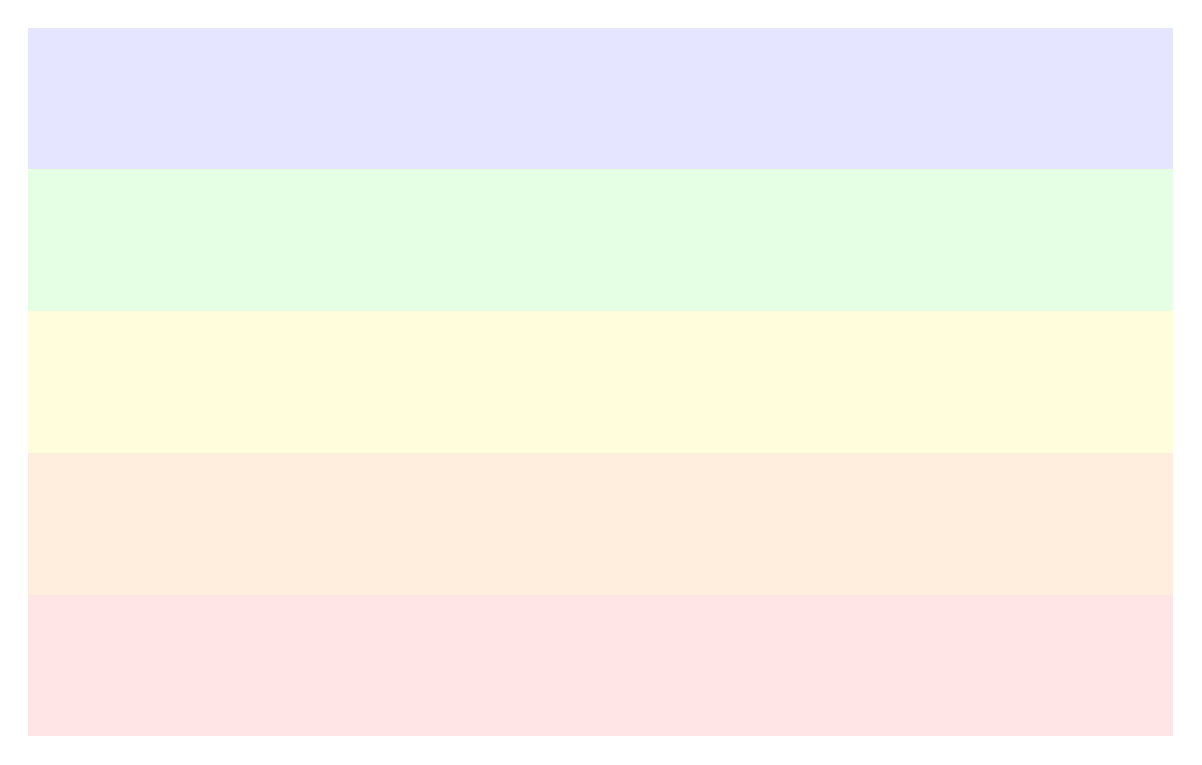
\begin{tikzpicture}[xscale=1.2, yscale=1.8]
\foreach \x/\y/\z in {0/red/10,1/orange/13,2/yellow/14,3/green/10,4/blue/10} {
  \path [fill=\y!\z] (0,\x) rectangle +(\textwidth,1);
}
\end{tikzpicture}$}


\setbeamertemplate{frametitle}{\color{black}\centering\Huge\bfseries\insertframetitle\par\vskip-6pt}

\begin{frame}
\frametitle{OUR QUANTUM WORLD}
- EVERYDAY WORLD = CLASSICAL, TINIEST THINGS BEHAVE DIFFERENTLY.\\
-....\\
- WHAT CAN WE DO WITH THIS?
\end{frame}
\begin{frame}
\frametitle{QUANTUM COMPUTERS}

\begin{minipage}{0.5\textwidth}\raggedright
Scientists around the world are racing to build the first \textit{quantum computer}.
\end{minipage}
\begin{minipage}{0.4\textwidth}\raggedright
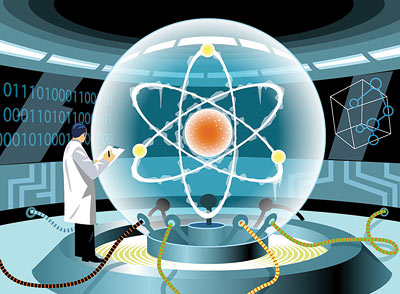
\includegraphics[height=3cm]{images/quantum_atom_in_room.png}
\end{minipage}

\vspace{15pt}
Over the next 100 years, they will transform our civilization, giving us incredible new powers of ... DRUG DESIGN, OPTIMIZATION, DATA ANALYSIS, BREAKING ENCRYPTION, ARTIFICIAL INTELLIGENCE. [INSERT PICTURES FROM DALHOUSIE TALK.]

\vspace{15pt}
Today we will investigate some of the basic principles of quantum computers.

\end{frame}

\newcommand\col[2]{\begin{minipage}{#1\textwidth}\raggedright #2\end{minipage}}


\begin{frame}
\frametitle{QUANTUM COMPUTERS ARE STRANGE}
- quantum mechanics is strange --> quantum computers are strange.\\
- entanglement
-superposition\\
- teleportation.
\end{frame}
\begin{frame}
\frametitle{QUBITS}
\vspace{25pt}
\col{0.5}{
Ordinary computers are built from \textit{bits}, which can equal 0 or 1.

\vspace{25pt}
Quantum computers will be built from \textit{qubits}. You've got one in front of you!

\vspace{25pt}
It has got lots of mysterious buttons.
\\
Give them a try.

\vspace{25pt}
We will use these buttons to tell the qubit what to do.
}
\col{0.4}{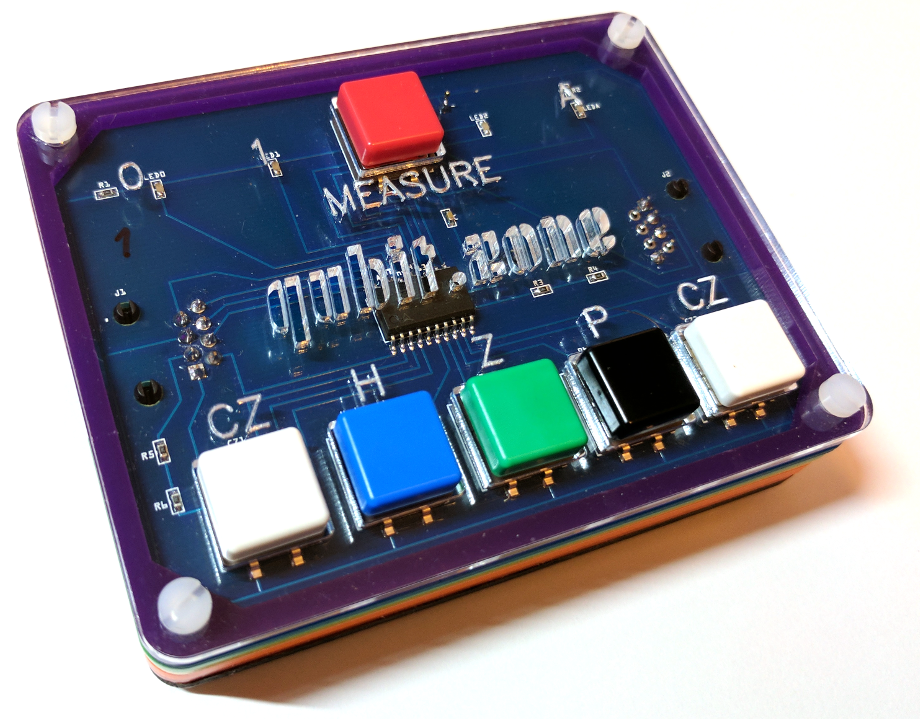
\includegraphics[height=6cm]{images/qubit_1.png}}

\end{frame}

\begin{frame}
\frametitle{SUPERPOSITION}

In the everyday world, ...EITHER OR

\vspace{20pt}
Schr\"odinger's cat\\

M button = looking into schr\"odinger's box.

Measurement and collapse\\

Be clear: If you press H then M repeatedly, get any number that you want.

\end{frame}

\begin{frame}
\frametitle{QUANTUM PROGRAMS}
\vspace{25pt}
A \textit{quantum program} is a recipe which tells you which buttons have to be pressed in which order. Here's an example:
\vspace{25pt}
\[ 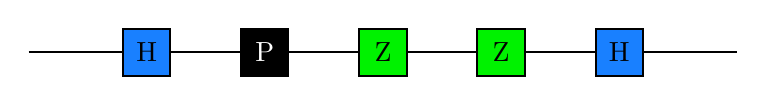
\begin{tikzpicture}[xscale=3]
\draw[string](0,0) to +(3,0);
\node[H] at (0.5,0) {H};
\node[P] at (1,0) {P};
\node[Z] at (1.5,0) {Z};
\node[Z] at (2,0) {Z};
\node[H] at (2.5,0){H};
\end{tikzpicture}
\]

\vspace{10pt}Usually, quantum programs use more than one qubit:
\vspace{10pt}
\[ 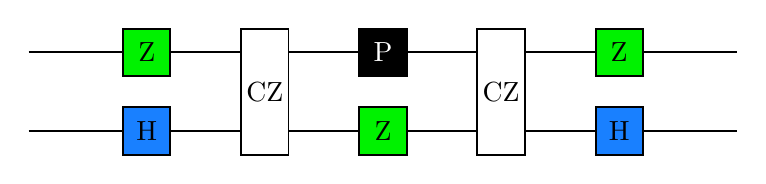
\begin{tikzpicture}[xscale=3]
\draw[string] (0,0) to + (3,0);
\draw[string] (0,1) to + (3,0);
\node[H] at (0.5,0) {H};
\node[Z] at (0.5,1) {Z};
\node[P] at (1.5,1) {P};
\node[Z] at (1.5,0) {Z};
\node[Z] at (2.5,1) {Z};
\node[H] at (2.5,0){H};
\node[CZ={1}] at (2,0.5) {CZ};
\node[CZ={1}] at (1,0.5) {CZ};
\end{tikzpicture}
\]
\end{frame}

\begin{frame}
\frametitle{ENTANGLEMENT}
Physics\\
- spooky action, immediate 'faster than light'.\\
-make it sound cool.
\end{frame}
\begin{frame}
\frametitle{ENTANGLEMENT}

\begin{columns}[t]
\column{0.5\textwidth}{
Let's entangle two qubits! Press \inlineH then \\[5pt]\inlineM on your qubit until you get ``0".
}
\column{0.5\textwidth}{
Get into pairs and entangle your qubits: }
\end{columns}

\vspace{10pt}

\[ 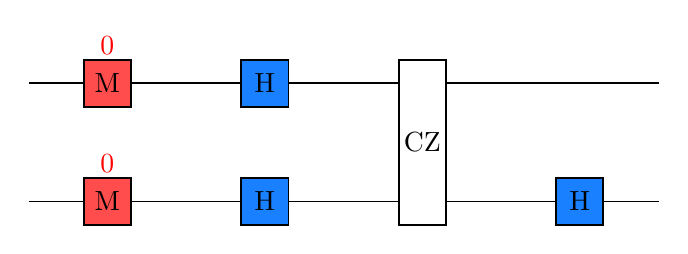
\begin{tikzpicture}[xscale=2]
\draw[string] (-0.5,0) to + (4,0);
\draw[string] (-0.5,1.5) to + (4,0);
\node[H] at (1,0) {H};
\node[H] at (1,1.5) {H};
\node[H] at (3,0){H};
\path (0,1.5) node [M] {M} node [result] {0};
\path (0,0) node [M] {M} node [result] {0};
\node[CZ={1.5}] at (2,0.75) {CZ};
\end{tikzpicture}
\]

\vspace{20pt} Your qubits are now entangled - measuring one of them will yield the same result as measuring the other one.

%Make clear that if you do anything with the qubits after you've measured them, the entanglement is broken.

\end{frame}

\begin{frame}
\frametitle{DENSE CODING}
\end{frame}

\begin{frame}
\frametitle{SENDING NUMBERS}

Imagine you wanted to send your friend a ``0'' or a ``1''.

\vspace{7pt}
\textit{Could you do this using a qubit?}

\vspace{20pt}
Yes! Just press \inlineH then \inlineM until you get the number you want.

\vspace{7pt}
Then pass the qubit to your friend.

\vspace{7pt}
They can press \inlineM to discover the message.

\vspace{25pt}
\textbf{Let's try it!}

\vspace{20pt}
Could you send your friend \emph{two numbers} by passing them one qubit?

\end{frame}

\tikzset{top note/.style={align=center, above=0.35cm, font=\it}}

\begin{frame}
\frametitle{SENDING NUMBERS}
\begin{columns}[t]
\column{0.45\textwidth}{%
With entanglement, you can use \textit{one} qubit to send \textit{two} numbers.\\
 Get into pairs. Choose who will be the sender and receiver.

}
\column{0.5\textwidth}{%
The sender secretly chooses a first number (0 or 1), and a second number (0 or 1).


}
\end{columns}


\[
\def\scl{0.8}
\begin{tikzpicture}[scale=\scl, rotate=-90, every node/.style={rotate=0}]
\def\xgap{2.8}
\draw [string] (0,-0.5) to (0,5) to [out=up, in=down, looseness=0.5] node [align=center, sloped, font=\it] {give qubit to\\[-2pt]your friend} (\xgap-1,7) to +(0,3.5);
\draw [string] (\xgap,-0.5) to (\xgap,10.5);
\node [Z] at (0,0.5) {Z};
\node [top note] at (0,4.5) {only if second\\[-1pt]number is 1};
\node [H] at (0,2.5) {H};
\node [Z] at (0,4.5) {Z};
\node [top note] at (0,0.5) {only if first\\[-1pt]number is 1};
\draw [string, dashed] (0,-0.5) to +(0,-0.75);
\draw [string, dashed] (\xgap,-0.5) to +(0,-0.75);
\node [align=center, font=\it] at (0.5*\xgap,-0.9) {start with a pair of\\[-1pt]entangled qubits};
\node [CZ ={\scl}] at (\xgap-0.5,7.5) {CZ};
\node [H] at (\xgap,9.) {H};
\node [H] at (\xgap-1,9) {H};
\node [M] at (\xgap,10.5) {M};
\node [M] at (\xgap-1,10.5) {M};
\draw[dashed,->] (\xgap-1, 11.2) to +(0,0.5);
\draw[dashed,->] (\xgap, 11.2) to +(0,0.5);
\node[align=center, font=\it, right=0.01cm] at (\xgap-1, 11.7) {2nd number};
\node[align=center, font=\it, right=0.01cm] at (\xgap, 11.7) {1st number};
\end{tikzpicture}
\]
\vspace{-1cm}

\end{frame}

\begin{frame}
\frametitle{TELEPORTATION IS COOL}
- entangelemet: Magically one qubit knows everything about another qubit/\\
- exciting story.
- Star Trek\\
- perfectly send stuff.\\

\end{frame}
\begin{frame}
\frametitle{TELEPORTATION}

Get into pairs and entangle your qubits. \\
??
\tikzset{bottom note/.style={align=center, below=0.35cm, font=\it}}
\[
\begin{tikzpicture}
\def\ygap{2.5}
\draw[string] (-2,0) to +(5,0);
\draw[string] (-1,-1) to + (4,0);
\draw[string,dashed] (-2,-1) to +(1,0);
\draw[string,dashed] (-2,-1-\ygap) to +(1,0);
\draw[string] (-1,-1-\ygap) to + (10,0);
\node[CZ={1}] at (0.,-0.5) {CZ};
\node[H] at (1.5,-1) {H};
\node[H] at (1.5,0) {H};
\node[M] at (3,0) {M};
\node[M] at (3,-1) {M};
\node[Z] at (5,-1-\ygap) {Z};
\node[H] at (6.5,-1-\ygap) {H};
\node[Z] at (8,-1-\ygap) {Z};
\draw[dashed,->] (3.6,-1) to [out = right, in=up, looseness=0.9] (5,-0.4-\ygap);
\draw[dashed,->] (3.6,0) to [out = right, in=up, looseness=1.2] (8,-0.4-\ygap);
\node [align=center, font=\it] at (-1.5,-1-0.5*\ygap) {start with a pair of\\[-1pt]entangled qubits};
\draw[dashed, ->] (-3,0) to (-2.5,0);
\node[align=center, font=\it] at (-4,0) {your qubit};
\node[align=center,font=\it,rotate=20] at (6, -1-0.2*\ygap) {tell your friend your \\[-2pt] measurement outcomes};

\node [bottom note] at (5,-1-\ygap) {only if this\\[-1pt]outcome was 1};
\node [bottom note] at (8,-1-\ygap) {only if this\\[-1pt]outcome was 1};
\end{tikzpicture}
\]

\end{frame}

\begin{frame}
\frametitle{GHZ?}

\[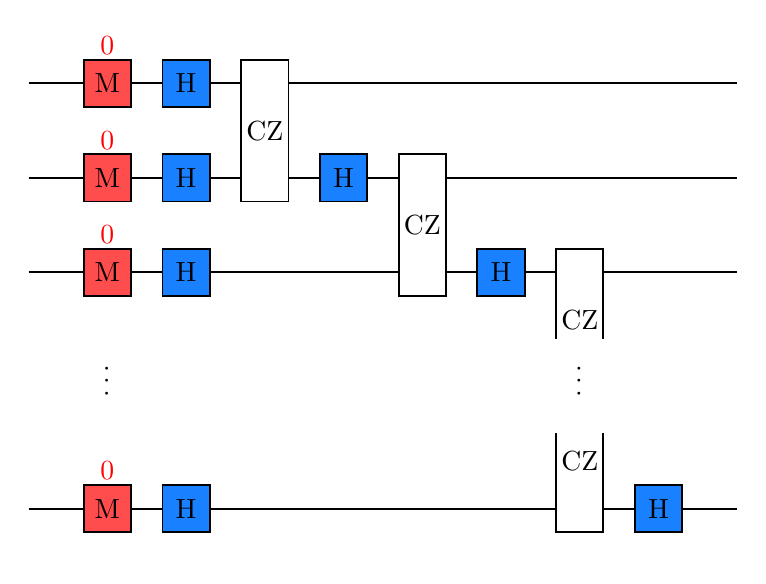
\begin{tikzpicture}
\def\ygap{1.2}
\draw[string] (0,0) to +(9,0);
\draw[string] (0,-\ygap) to + (9,0);
\draw[string] (0,-2*\ygap) to +(9,0);
\node[rotate=90] at (1,-3.15*\ygap){$\cdots$};
\draw[string] (0,-4.5*\ygap) to +(9,0);
\path (1,0) node [M] {M} node [result] {0};
\path (1,-\ygap) node [M] {M} node [result] {0};
\path (1,-2*\ygap) node [M] {M} node [result] {0};
\path (1,-4.5*\ygap) node [M] {M} node [result] {0};
\node[H] at (2,0) {H};
\node[H] at (2,-\ygap) {H};
\node[H] at (2,-2*\ygap) {H};
\node[H] at (2,-4.5*\ygap) {H};
\node[CZ={\ygap}] at (3, -0.5*\ygap) {CZ};
\node[H] at (4, -\ygap) {H};
\node[CZ={\ygap}] at (5,-1.5*\ygap) {CZ};
\node[H] at (6, -2*\ygap) {H};
\begin{scope}
\clip (0,0) rectangle (8, -2.7*\ygap);
\node[CZ={\ygap}] at (7,-2.5*\ygap) {CZ};
\end{scope}
\node[rotate=90] at (7,-3.15*\ygap){$\cdots$};
\begin{scope}
\clip (0, -5*\ygap) rectangle (8, -3.7*\ygap);
\node[CZ ={\ygap}] at (7,-4*\ygap){CZ};
\end{scope}
\node[H] at (8, -4.5*\ygap) {H};

\end{tikzpicture}
\]
\end{frame}


\begin{frame}
\frametitle{That's what a quantum computer is!}
-maybe big composed circuit.
\end{frame}





\end{document}\end{document}\end{document}

\begin{frame}
\section{Qubits}

\paragraph{What is a qubit?}

Scientists around the world are racing to build the first quantum computer, which will use the laws of quantum mechanics to solve some problems much faster than any computer we have now. Using your very own qubit, we can investigate some of the 

While today's computers store information using bits, quantum computers will store information using qubits

...

 - A qubit is the basic building block of a quantum computer
 
 - Measure, one-qubit operations, two-qubit operations
 
 - Using the cable
 
 - All the operations cancel themselves out if you do them twice. So if you press one by accident, press it again
 
 \section{Measurement}
 
You can ask a qubit the following question: ``what state are you in?''. The answer will be 0 or 1.

\section{Superposition}



\section{Entanglement}

Two entangled qubits will behave the same way, however far separated they are in space.

\paragraph{Experiment.} Entangle two qubits, then measure each of them.

\section{Teleportation}

\paragraph{Experiment.} 

\section{Super Dense Coding}

We can use qubits to send messages, by 

\end{frame}

\end{document}


\begin{frame}
\frametitle{Teleport entangled states.}
\vspace{5pt}
\tikzset{bottom note/.style={align=center, below=0.35cm, font=\it}}
\[
\begin{tikzpicture}
\def\ygap{2.5}
\draw[string] (-1,0.8*\ygap) to +(10,0);
\draw[dashed] (-2,0) to +(1,0);
\draw[dashed] (-2,0.8*\ygap) to +(1,0);
\node [align=center, font=\it] at (-1.5,0.5*0.8*\ygap) {start with a pair of\\[-1pt]entangled qubits};
\draw[string] (-1,0) to +(4,0);
\draw[string] (-1,-1) to + (4,0);
\draw[string,dashed] (-2,-1) to +(1,0);
\draw[string,dashed] (-2,-1-\ygap) to +(1,0);
\draw[string] (-1,-1-\ygap) to + (10,0);
\node[CZ={1}] at (0.,-0.5) {CZ};
\node[H] at (1.5,-1) {H};
\node[H] at (1.5,0) {H};
\node[M] at (3,0) {M};
\node[M] at (3,-1) {M};
\node[Z] at (5,-1-\ygap) {Z};
\node[H] at (6.5,-1-\ygap) {H};
\node[Z] at (8,-1-\ygap) {Z};
\draw[dashed,->] (3.6,-1) to [out = right, in=up, looseness=0.9] (5,-0.4-\ygap);
\draw[dashed,->] (3.6,0) to [out = right, in=up, looseness=1.2] (8,-0.4-\ygap);
\node [align=center, font=\it] at (-1.5,-1-0.5*\ygap) {start with a pair of\\[-1pt]entangled qubits};

\node[align=center,font=\it,rotate=20] at (6, -1-0.2*\ygap) {tell your friend your \\[-2pt] measurement outcomes};

\node [bottom note] at (5,-1-\ygap) {only if this\\[-1pt]outcome was 1};
\node [bottom note] at (8,-1-\ygap) {only if this\\[-1pt]outcome was 1};
\end{tikzpicture}
\]
\end{frame}
